\documentclass[12pt,letterpaper,noanswers]{exam}
\usepackage[usenames,dvipsnames,svgnames,table]{xcolor}
\usepackage[margin=0.9in]{geometry}
\renewcommand{\familydefault}{\sfdefault}
\usepackage{multicol}
\pagestyle{head}
\definecolor{c03}{HTML}{FFDDDD}
\header{AM 108 Class 04}{Updated on \today.}{Bifurcations,  p. \thepage}
\runningheadrule
\headrule
\usepackage{graphicx} % more modern
\usepackage{amsmath} 
\usepackage{amssymb} 
\usepackage{hyperref}
\usepackage{tcolorbox}

\begin{document}
 \pdfpageheight 11in 
  \pdfpagewidth 8.5in

\vspace{0.2cm}

\hrule
\vspace{0.2cm}

\begin{itemize}
    \item There is a problem set due Friday at 5pm (submit via Gradescope).
    \item There is a skill check today.  The next one will be next Monday (with skills from C04/05/06).
    \item There is a pre-class assignment for Wednesday.
    \item OH this week: Tuesday 9:30-10am, 12:30-1pm, 4-4:30pm with Sarah.  Wednesday 7-8:30pm with Isaac.  Thursday 11-11:30am with Sarah, Thursday 3-4:30pm with P\'etur, Friday 11:30-noon with Sarah.
    
    Find more info on Canvas (top of the first page).  
    
    Before attending OH, \textbf{post} to \#officehours on Slack (or the Office Hours thread on Piazza).  This lets the course staff know you are attending and lets your classmates and instructors know what questions / problems you're bringing to OH.
\end{itemize}

\hrule
\vspace{0.2cm}

\noindent \textbf{Extra vocabulary / extra facts:}
\begin{tcolorbox}
\begin{itemize}
\item \textbf{continuation}: Let $x^*$ be an equilibrium of $\frac{dx}{dt} = f(x; r^*)$ where $f$ is continuous and differentiable, and $x^*$ is linearly stable (or unstable).  There there is a branch of equilibria, $x(r)$, with the same stability as $x^*$.  This branch exists for all $r$ sufficiently near $r^*$ .  [definition from Prof Ghrist ADS video textbook]

\item This is a ``linear'' intuition: small changes in $r$ lead to small changes in the location of the fixed points and no change in their stability.

\item A \textbf{local bifurcation} occurs at an equilibrium $(x^*, r^*)$ if, in any neighborhood of $(x^*, r^*)$, there is a change in the number or types of equilibria.  A necessary condition for a bifurcation is that $\left.\frac{df(x; r^*)}{dx}\right\vert_{x^*} = 0$ (or that $\left.\frac{\partial f(x; r)}{\partial x}\right\vert_{(x^*,r^*)} = 0$).
[definition from Prof Ghrist ADS video textbook]

\item At a \textbf{pitchfork bifurcation}, two new fixed points are created at the moment of bifurcation.  If these new fixed points are stable, the bifurcation is called \textbf{supercritical}.  If they are unstable, it is called \textbf{subcritical}.

\item The name of the \textbf{saddle-node bifurcation} will make more sense in higher dimensions, where a type of fixed point called a \textbf{saddle point} collides with a type of fixed point called a \textbf{node} at the point of bifurcation.
\end{itemize}

\end{tcolorbox}

\noindent Note: Away from bifurcation points, fixed points of the system are typically hyperbolic (linear stability analysis tells us the stability of the fixed point).  At the point of bifurcation (the parameter value associated with the bifurcation), there is a non-hyperbolic fixed point.

\vspace{0.2cm}

\hrule
\vspace{0.2cm}
\eject

\noindent\textbf{Comments/questions}

General bifurcation topics
\begin{enumerate}
\itemsep-0.2em
\item What is the difference between $\dot x$ and $f'(x)$?
\item More examples / practice + a workflow for generating the diagrams.
\item What happens when we take $\dot{x} = f(x; r)$, set $f(x; r) = 0$, and can't find an explicit formula $x = g(r)$ that corresponds to $f(x; r) = 0$?
\item When is the branch of fixed points drawn with a solid line, vs with a dashed line?
\item How do we tell the different bifurcations apart?  How do the saddle-node and transcritical differ?
\item Note: the saddle-node and transcritical bifurcation points are half-stable.
\item Is it the case that all half-stable fixed points are caused by bifurcations?  
\item Exponential vs algebraic stability came up again.
\item ``I thought that our choice of [parameter] would impact the system independently to any previous choices..., but it seems that this assumption is wrong in light of subcritical bifurcation diagrams''
\item What exactly defines a normal form?
\end{enumerate}

%Section 3.1: saddle-node bifurcation.
%\begin{enumerate}
%\itemsep-0.2em
%%    \item When we draw fixed points as curves in $rx$-space, how do we decide which curves to draw dotted and which to draw solid?  
%%   \item How does the plot of $\dot x$ vs $x$ relate to the bifurcation diagram in $rx$-space?
%
%\end{enumerate}

Section 3.4: pitchfork bifurcation.
\begin{enumerate}
\itemsep-0.2em
%    \item When making a bifurcation diagram for $\dot x = rx - x^3$, why think of $x$ as the independent variable and $r$ as the dependent variable to make the plot in $rx$-space?
%    \item Where do the terms ``subcritical'' and ``supercritical'' come from?  Why do they ignore the change on the center line of the pitchfork and only refer to the extra branches?
 %   \item For $\dot x = r x + x^3 - x^5$, where there are multiple stable fixed points at a single value of $r$, where do `jumps' or `hysteresis' come in?
 \item In the box on a stick example, if the stick bends on its way to breaking, when is the moment of bifurcation?
 
\end{enumerate}

\vspace{4in}

\vspace{0.2cm}
\hrule
\vspace{0.2cm}

\noindent\textbf{Skill check C04 practice} (the skill check will have one question similar, but not identical, to the question below).


\begin{questions}
\item For each of the four bifurcation diagrams given below, name the bifurcation that occurs in the diagram.

%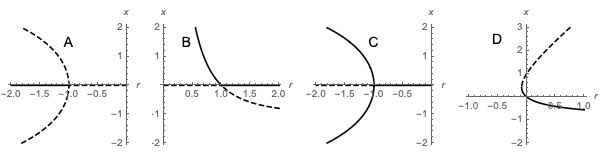
\includegraphics[width=\linewidth]{img/C04-2019-09-11bifn.png}
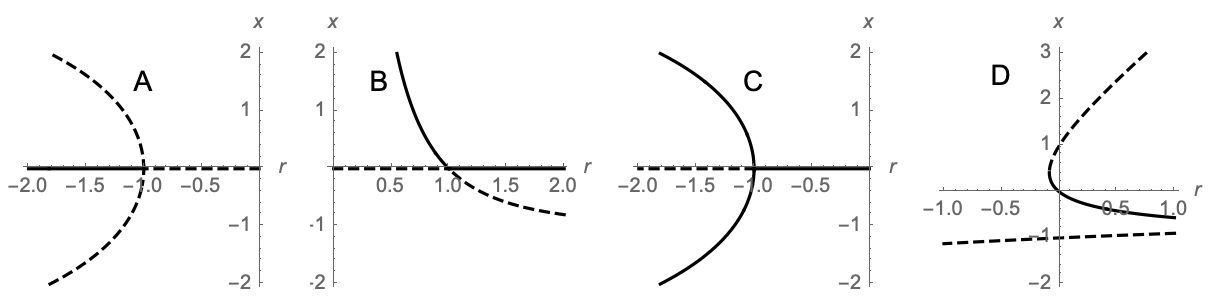
\includegraphics[width=\linewidth]{img/S22-bifurcation-skill.png}


\bgroup
\def\arraystretch{2}
\begin{tabular}{|l|p{10cm}|}
\hline
Plot     & \hspace{0.5cm} Bifurcation name \\
\hline\hline
 A    & \\
 \hline
 B & \\
 \hline
 C & \\
 \hline
 D & \\
 \hline
\end{tabular}
\egroup
\end{questions}

\vspace{0.2cm}
\hrule
\vspace{0.2cm}
\noindent\textbf{Skill check C04 practice solution} 

The possibilities are: saddle-node bifurcation, transcritical bifurcation, supercritical pitchfork bifurcation, subcritical pitchfork bifurcation.  There are all the bifurcations we have learned so far.

In (A) the bifurcation point is at $r = -1$.  Very close to the bifurcation there are three branches to one side and one to the other side.  The $x=0$ fixed point changes stability at the bifurcation and the two extra branches are both unstable.  This is a \emph{subcritical pitchfork bifurcation}.  (Subcritical because the extra branches are unstable).

In (B) the bifurcation point is at $r = 1$.  Very close to the bifurcation there are two branches to each side, so it is a \emph{transcritical bifurcation}.

In (C) the bifurcation point is at $r = -1$.  Very close to the bifurcation there are three branches to one side and one to the other side.  The $x=0$ fixed point changes stability at the bifurcation and the two extra branches are both stable.  This is a \emph{supercritical pitchfork bifurcation}.  (Supercritical because the extra branches are stable).

In (D) the bifurcation point is at $r$ a little less than $0$.  Looking very close to the bifurcation (in both $r$ and $x$ - imagine drawing a little circle right around the bifurcation) there are two branches on one side and no fixed points on the other side.  This is a \emph{saddle node bifurcation}.

\vspace{0.2cm}

\hrule
\vspace{0.2cm}








\noindent\textbf{Teams}

\begin{multicols}{3}
1. David, Arda, Siqi, Dmitry

2. Karla, Alia, Raelene

3. Stephen, Brián, Max

4. Haruka, Isha, Matthew

5. Cyrus, Sara, Richard

6. Eddie, Aaron, Jessica

7. Adam, Tara, Georgia

8. Vanesa, Ben, Isheka

9. Julio, Emma, Rosie, Soto

10. Ayla, Caroline, Nick

\end{multicols}

\noindent \textbf{Teams 3 and 7}: Post photos of your work to the course Google Drive today.  Include words, labels, and other short notes that might make those solutions useful to you or your classmates.  Find the link in Canvas.
\vspace{0.2cm}

\hrule
\vspace{0.2cm}
%\eject

\noindent\textbf{Team activity}

Write your names on your whiteboard before you begin.

Icebreaker: share a type of vegetable that you particularly enjoy


\begin{questions}


\item

% \begin{tcolorbox}
% Learning goal (procedural, factual): Follow the procedure described in the problem to create a bifurcation diagram.  Identify the type of bifurcation.
% \end{tcolorbox}



Think of \[\dot{x} = x(1+x)\] as being a member of the family of differential 
equations specified by \[\dot{x} = x(r+x).\]  (It is the differential equation that arises when $r=1$).  We'd like to understand all of the possible phase portraits that arise for this family of equations.  This is one purpose of a \textbf{bifurcation diagram}.  

For this problem, consider $r$ to be a parameter of the differential equation, $t$ to be the independent variable, and $x$ to be the dependent variable.

\begin{parts}
\item Find the fixed points of the differential equation as a function of $r$.  
% \begin{itemize}
% \item Does the number of fixed points vary with the value of $r$? 
% \item Given how the number of fixed points varies, could there be an isolated saddle-node bifurcation in this system?  What about a transcritical bifurcation or a pitchfork bifurcation?  Discuss your reasoning.
% \end{itemize}
\item Choose one of your fixed points and use linear stability analysis to identify its stability as a function of $r$.  Use your knowledge of vector fields and phase portraits to reason out the stability of the other fixed point (without calculation).
\item Create a bifurcation diagram showing the values of the fixed points vs $r$.  Indicate the stability of the fixed points with solid lines for stable points and dashed lines for unstable fixed points.
\item A bifurcation occurs at a particular parameter value where the phase portrait undergoes a qualitative change.  Identify $r_c$, the critical value of the parameter at the bifurcation.
\item What type of bifurcation is this?
\end{parts}

% Stop here.  If a number of other groups are still working, spread out, with each of you visiting a different team.  Introduce yourself and see what you can learn from how they are working on the problem. 


\item Last time we worked with the dynamical system given by $\dot{x} = x/2 - \tanh x$.  (We also looked at the system $\dot{x} = \tanh x - x/2$).  Now consider the differential equation
\[\dot{x} = r x - \tanh x.\]  Recall that $\tanh(x) = \frac{e^x-e^{-x}}{e^x+e^{-x}}.$
\begin{parts}
\item Last week you worked with the case $r=1/2$ to find the phase portrait.  Now we'll consider what happens as $r$ changes.  Identify the qualitatively different phase portraits that can occur for different values of $r$.
\item  Argue that a bifurcation occurs and identify the type of bifurcation (including, if relevant, whether
it is subcritical or supercritical).
\item One fixed point is not hard to identify.  Use linear stability analysis on this fixed point to find $r_c$, the critical value of the parameter at the bifurcation (this is the value of $r$ where the fixed point becomes non-hyperbolic).
\item Sketch the bifurcation diagram.  It is just fine to give a rough approximation of how you think it looks.


% The following Mathematica/Wolframalpha command will help you find the actual shape.  Identify what this command is doing and discuss why it would give you the shape of the bifurcation diagram.
% \begin{verbatim}
% ContourPlot[r x - Tanh[x]==0, {r,-1,2},{x,-2,2}]
% \end{verbatim}
\end{parts}
\end{questions}

% 2018: many groups got to here but not all.  We switched to problems at 1:50pm, so 43 minutes into class.
% 2019: most groups got to here and I posted a solution to piazza.
\vfill

% \noindent Extra Question:
% \begin{questions}
% \item (3.4.14) Consider the system $\dot{x} = r x + x^3 - x^5$.  
% \begin{parts}
% \item Find an algebraic expression for each of the fixed points as $r$ varies.  \emph{You'll have a 4th order polynomial to deal with, but you can let $\xi = x^2$ and treat the polynomial as a quadratic in $\xi$.}
% \item Calculate $r_s$, the parameter value at which the nonzero fixed points are born in a
% saddle-node bifurcation.
% \item Sketch the bifurcation diagram.
% \end{parts}

%\question (Potential functions)  We have been analyzing first order systems $\dot{x} = f(x)$ by identifying fixed points.  Sometimes the idea of a \emph{potential function} is used as well.  This is a function $V(x)$ such that $\displaystyle\dot{x} = -\frac{dV}{dx}$.  The name ``potential function'' comes to us from physics.  
%\begin{parts}
%\part A potential function $V(x)$ associated with the system $\dot{x} = -x$ is $V(x) = \frac{1}{2}x^2$.  Sketch the potential function.  Identify the location of the stable fixed point along the $x$-axis.  How does $V(x)$ look near the stable fixed point?
%\part An interesting fact about potential functions is that $\frac{dV}{dt}\leq 0$ along a solution curve $x(t)$.  This means that a particle moving under the action of the flow can only move in such a way that $V$ decreases or stays the same.  
%
%To show this, Use the chain rule on $\frac{dV}{dt}$ to write it in terms of $\frac{dV}{dx}$.  On trajectories, we know $\dot{x} = -\frac{dV}{dx}$ by definition of the potential function.  
%
%Combine this information to argue that particles can only move in such a way that $V$ decreases or stays constant in time.
%
%\part Consider $\dot{x} = r - x^2$.  Find a potential function.  Sketch the potential function for a few values of $r$.  Include the qualitatively different cases.  Mark the locations of the fixed points along the $x$-axis.
%\end{parts}
%\end{questions}

\end{document}